\section{Background}
\label{sec:background}
In this section, we give an overview of the differences between HTTP/2 over TCP and QUIC and introduce the QoE metrics we use to evaluate the performance of a variety of ABR streaming approaches. This is followed by an overview of our retransmission scheduling approach described in ~\cite{Wang:TOMM:2017}.

\subsection{QUIC vs. TCP}
\label{subsubsec:quicvstcp}
With the advent of QUIC there are now two options for the transport of HTTP/2 sessions between a web server and a browser. First, the original approach specifies the use of HTTP/2 over TCP. The second approach involves QUIC as an additional application layer protocol, which results in a HTTP/2 over QUIC over UDP solution~\cite{quic_chromium}.

TCP requires a 3-way handshake resulting in a 1.5 RTT before any data request is received at the server. In the case of QUIC, the data request arrives after 0.5 RTT at the server.

The default congestion control algorithm implemented in QUIC is similar to that of TCP Cubic \cite{ha2008cubic} with some important differences.
In order to notify the sender of the train of packets received, existing TCP mechanisms (including CUBIC) make use of Selective Acknowledgements (SACK) that include a maximum of the 3 most recent sequential packets that arrived successfully. The sender then retransmits the lost packets with sequence numbers that lie within the range of the 3 SACKs received. It is obvious that this approach imposes a heavy constraint on the number of TCP retransmissions that can take place without response from the receiver. QUIC aims to resolve this by including the use of NACKs and allows the receiver to send up to 256 NACKs without waiting for a response from the sender. The use of NACKs allows much faster loss recovery and can lead to asignificant reduction in rebuffering at DASH clients.

\subsection{QoE metrics for ABR Streaming}
For the evaluation of the performance of ABR streaming applications we make use of the following metrics, which are widely used in related work:
%The following metrics are generally accepted for measuring the QoE of ABR Streaming applications:

\hfill \break
{\bf Average Quality Bitrate ($AQB$):} One of the objectives of quality adaptation algorithms is to maximize the average quality bitrate of the streamed video. For a comprehensive QoE representation, we need to combine this metric with the {\it Number of Quality Switches} which is explained below.
\hfill \break
{\bf Number of Quality Switches ($\#QS$):} This metric is used together with $AQB$ to draw quantitative conclusions about the perceived quality (QoE). For example, for two streaming sessions having the same $AQB$, the session with the lower $\#QS$ will be perceived better by the viewer~\cite{ZinkSpectrum2005}.
\hfill \break
{\bf Spectrum ($H$) \cite{ZinkSpectrum2005}:} The spectrum of a streamed video is a centralized measure for the variation of the video quality bitrate around the $AQB$. A lower $H$ indicates a better QoE.
\hfill \break
{\bf Rebuffering Ratio ($RB$):} The average rebuffering ratio is given by the following equation:
\begin{equation}
\label{eq:rebuffer_ratio}
    RB = \mathsf{E}\left[\frac{t_a - t_e}{t_e}\right],
\end{equation}
Where $t_a$ is the actual playback time and $t_e$ is the video length in seconds, respectively.

It is well known that low rebuffering and high average quality bitrate are highly desirable for an optimal QoE. In our previous work \cite{Wang:TOMM:2017}, we show that reducing quality gaps through ABR segment retransmissions can contribute significantly to a higher $AQB$. In the following, we present an analysis of actual quality gaps that occur in a real-world trace.
\subsection{Segment retransmission scheduling}
\label{subsec:retrans_sched}

Traditional ABR approaches stream the ABR video segments in the order provided by the MPD file. Looking closely at the segment qualities buffered at the client at any point in time SQUAD shows that these reflect the recent quality decisions made by the adaptation algorithm, which, in turn, are based on the specific interpretation of the measured download rate and the corresponding buffer filling. Looking at the buffer filling in \emph{retrospect} as in Fig.~\ref{fig:retrans} (a) SQUAD identifies quality switches that are denoted as quality ``gaps". The emergence of these quality gaps is complex as it describes the instantaneous interaction of the adaptation algorithm with the buffer filling state and the download rate. In the following, we illustrate how to improve the QoE by filling some of these quality gaps. Fig.~\ref{fig:retrans} shows a simplified example of segment qualities inside the player buffer with different possible gaps. SQUAD defines gaps as the downward variation from the quality level which negatively impact the QoE~\cite{ZinkSpectrum2005}.

\begin{figure}
\centering
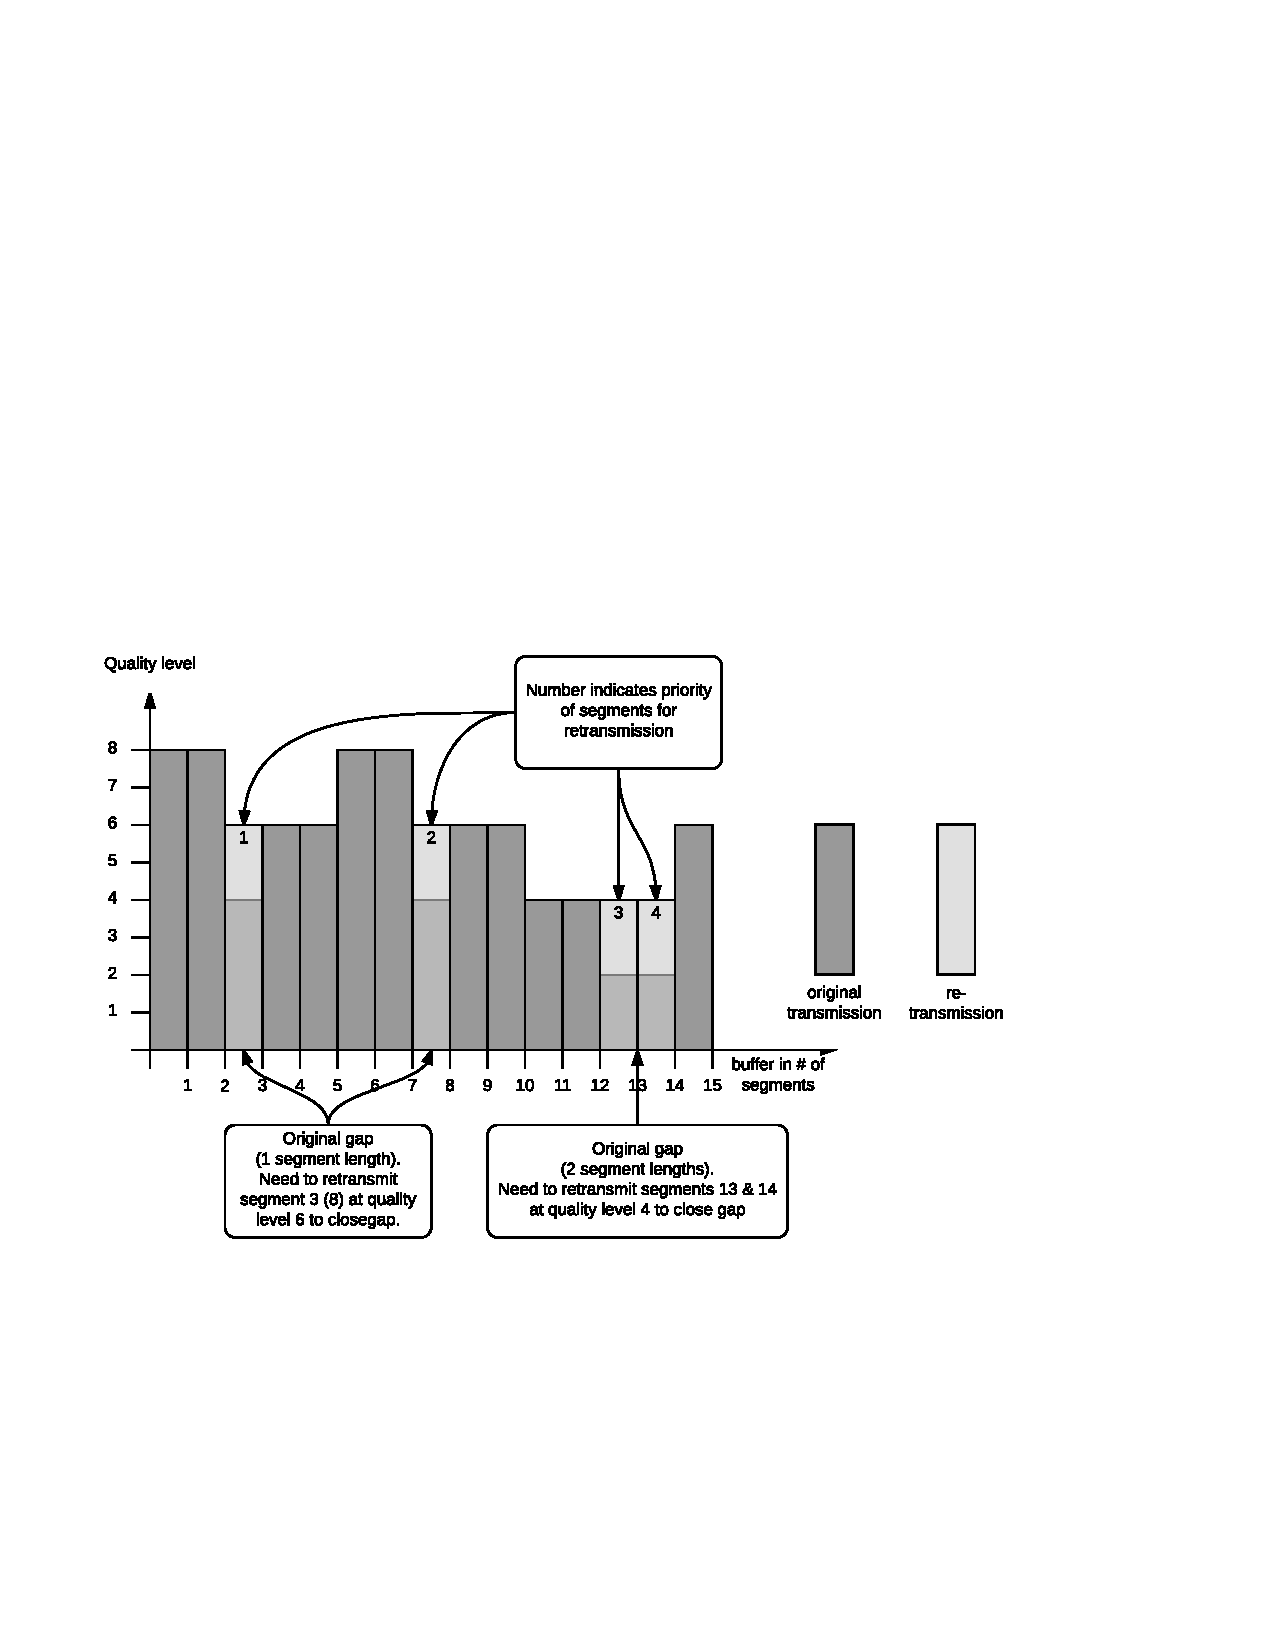
\includegraphics[width=.9\linewidth] {figures/Retrans_example.pdf}
% 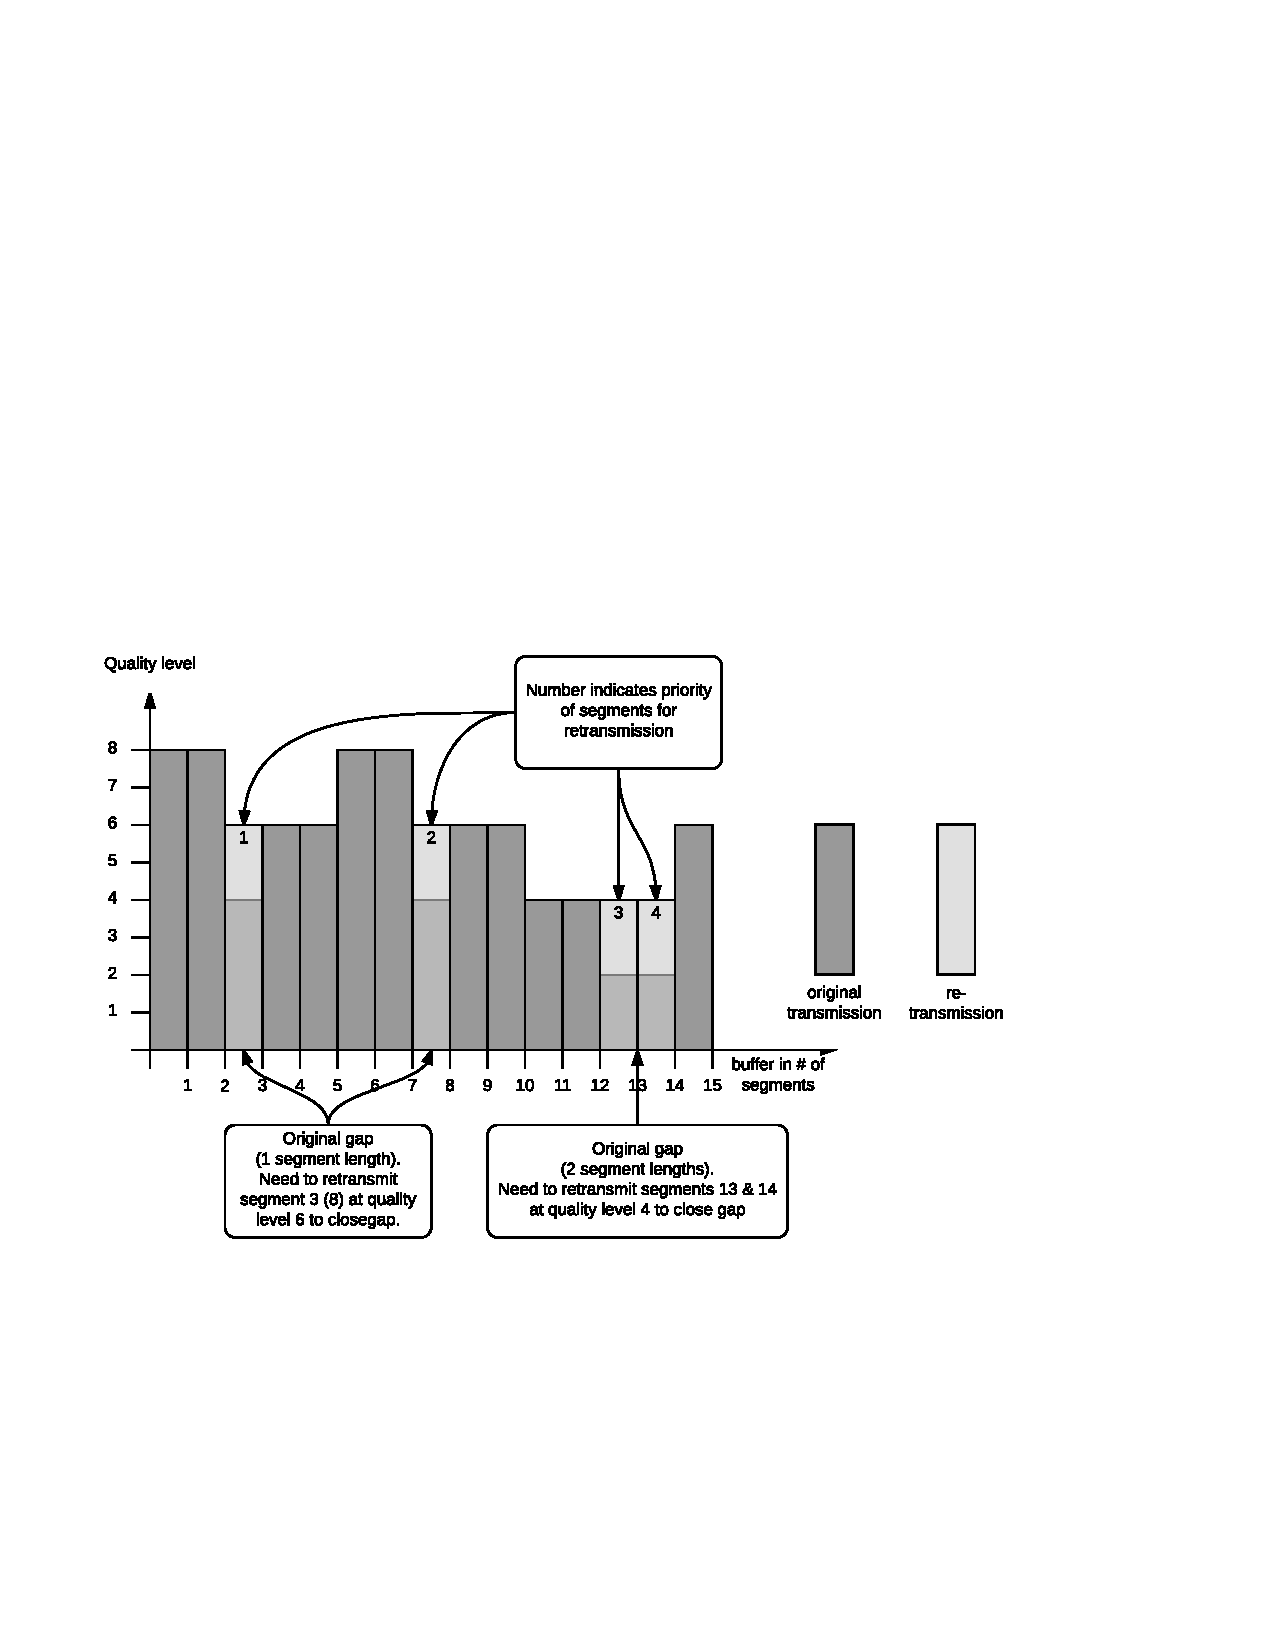
\includegraphics[scale=0.40, trim={0mm 100mm 0mm 90mm}] {figures/Retrans_example.pdf}
\caption{Example scenario for retransmissions. The QoE of this streaming session can be improved if, e.g., segments 3, 8, 13, and 14 are retransmitted in higher quality, assuming they arrive before their scheduled playout.}
\label{fig:retrans}
\vspace{-8pt}
\end{figure}

SQUAD's current approach is based on HTTP/1.1, which does not allow the parallel transmission of original segments and the retransmission of segments in a better quality. HTTP/2 over TCP allows this parallel transmission but does not prevent HOL blocking to efficiently perform retransmissions. In contrast, HTTP/2 over QUIC does not suffer from such inefficiencies and gives the application maximum control of individual streams and we show how this can be used to improve the QoE of ABR streaming.
\subsection{Analysis of Gaps in Streaming Sessions}
\label{subsec:ana_gap}
Akamai~\cite{AkamaiNetworkSIGOPS} is the world's largest CDN provider that delivers 15\%--30\% of global Internet traffic. Its CDN contains over 150,000 edge servers distributed in 90+ countries and 1200 ISPs around the world. To motivate the retransmission of segments as described in Sect.~\ref{subsec:retrans_sched}, we analyze an anonymized trace collected from Akamai's video CDN. This trace contains video streaming session information for a 3-day period in June 2014. The ABR streaming traffic in this trace contains 5 million video sessions originating from over 200,000 unique clients who were served by 1294 edge servers around the world. For each streaming session, each individual segment request is logged, which allows us to reconstruct the quality of the segments received at the client. Fig.~\ref{fig:gap_example} gives an example for one such streaming session we randomly picked for better illustration. As shown in Fig.~\ref{fig:gap_example}, this streaming session resulted in a  series of gaps. These gaps are potential candidates for segment retransmission that could lead to less quality level changes and, thus, an improve QoE. In Fig.~\ref{fig:gap_example}, we indicate that a retransmission of the segments in the later part of the stream could significantly impact the QoE.

\begin{figure}
\centering
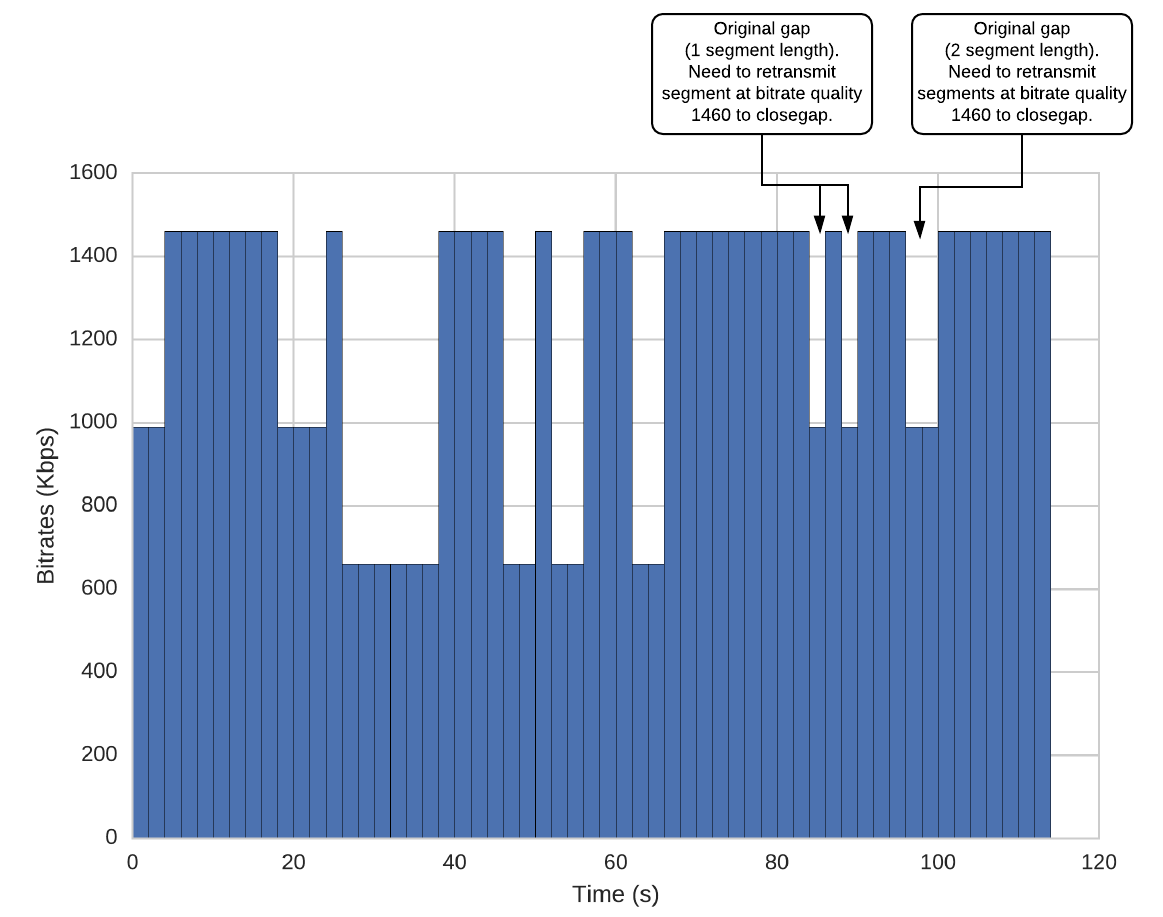
\includegraphics[width=.9\linewidth] {figures/mobonerun.png}
% 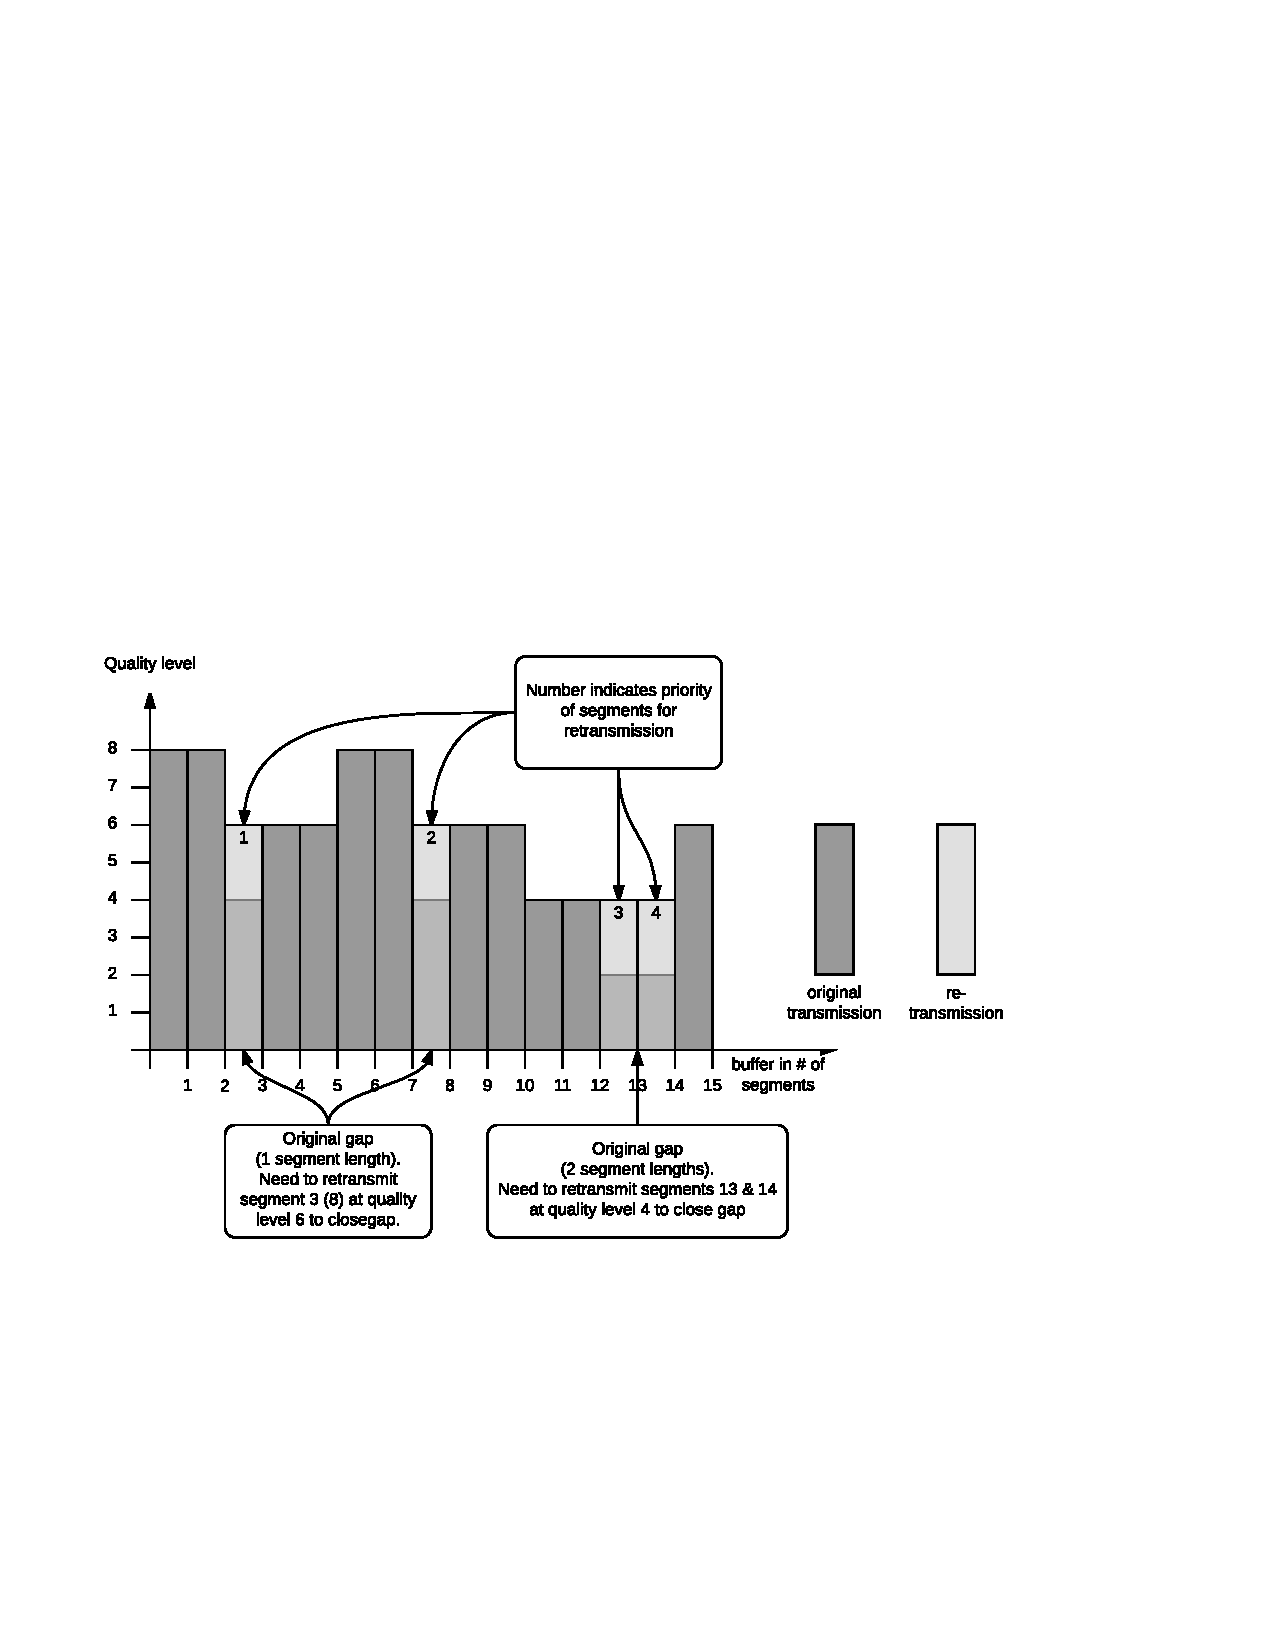
\includegraphics[scale=0.40, trim={0mm 100mm 0mm 90mm}] {figures/Retrans_example.pdf}
\caption{Original transmission of video stream from one randomly selected trace in the Akamai data set. The QoE of this video can be improved if the highlighted segments are retransmitted in higher quality, assuming they arrive before scheduled playout.}
\label{fig:gap_example}
\vspace{-18pt}
\end{figure}

In Fig.~\ref{fig:gap_cdf}, we show the results of our analysis for the complete data set which has approx. 5 million sessions, and for the a subset that only includes sessions for mobile devices, which has approx. 0.1 million sessions. This figure shows the percentage of sessions that have one or more gaps. Considering all sessions in the data set, 36.19\% of the sessions have at least one gap. These sessions could benefit from our segment retransmission approach. We also analyzed how many of the sessions with mobile clients have at least one gap. As shown in Fig.~\ref{fig:gap_cdf}, with 51.24\% this ratio is even higher. Obviously, this increase in sessions with at least one gap is not too surprising since mobile/wireless clients are assumed to experience higher bandwidth fluctuations than stationary/wired clients.

\begin{figure}
\centering
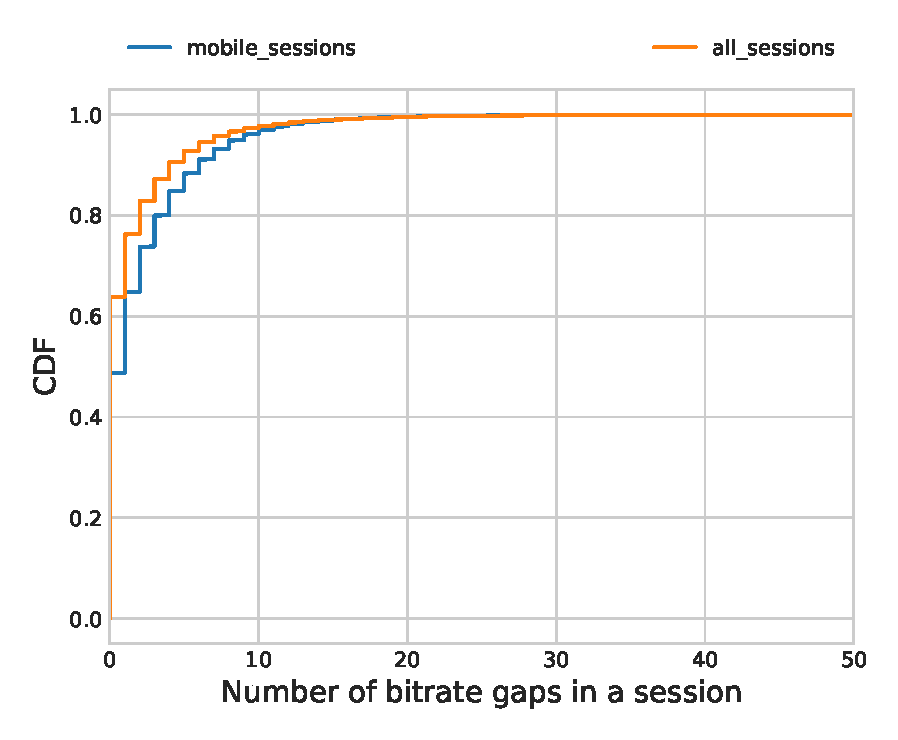
\includegraphics[width=.9\linewidth] {figures/all_gapCDF.eps}
% 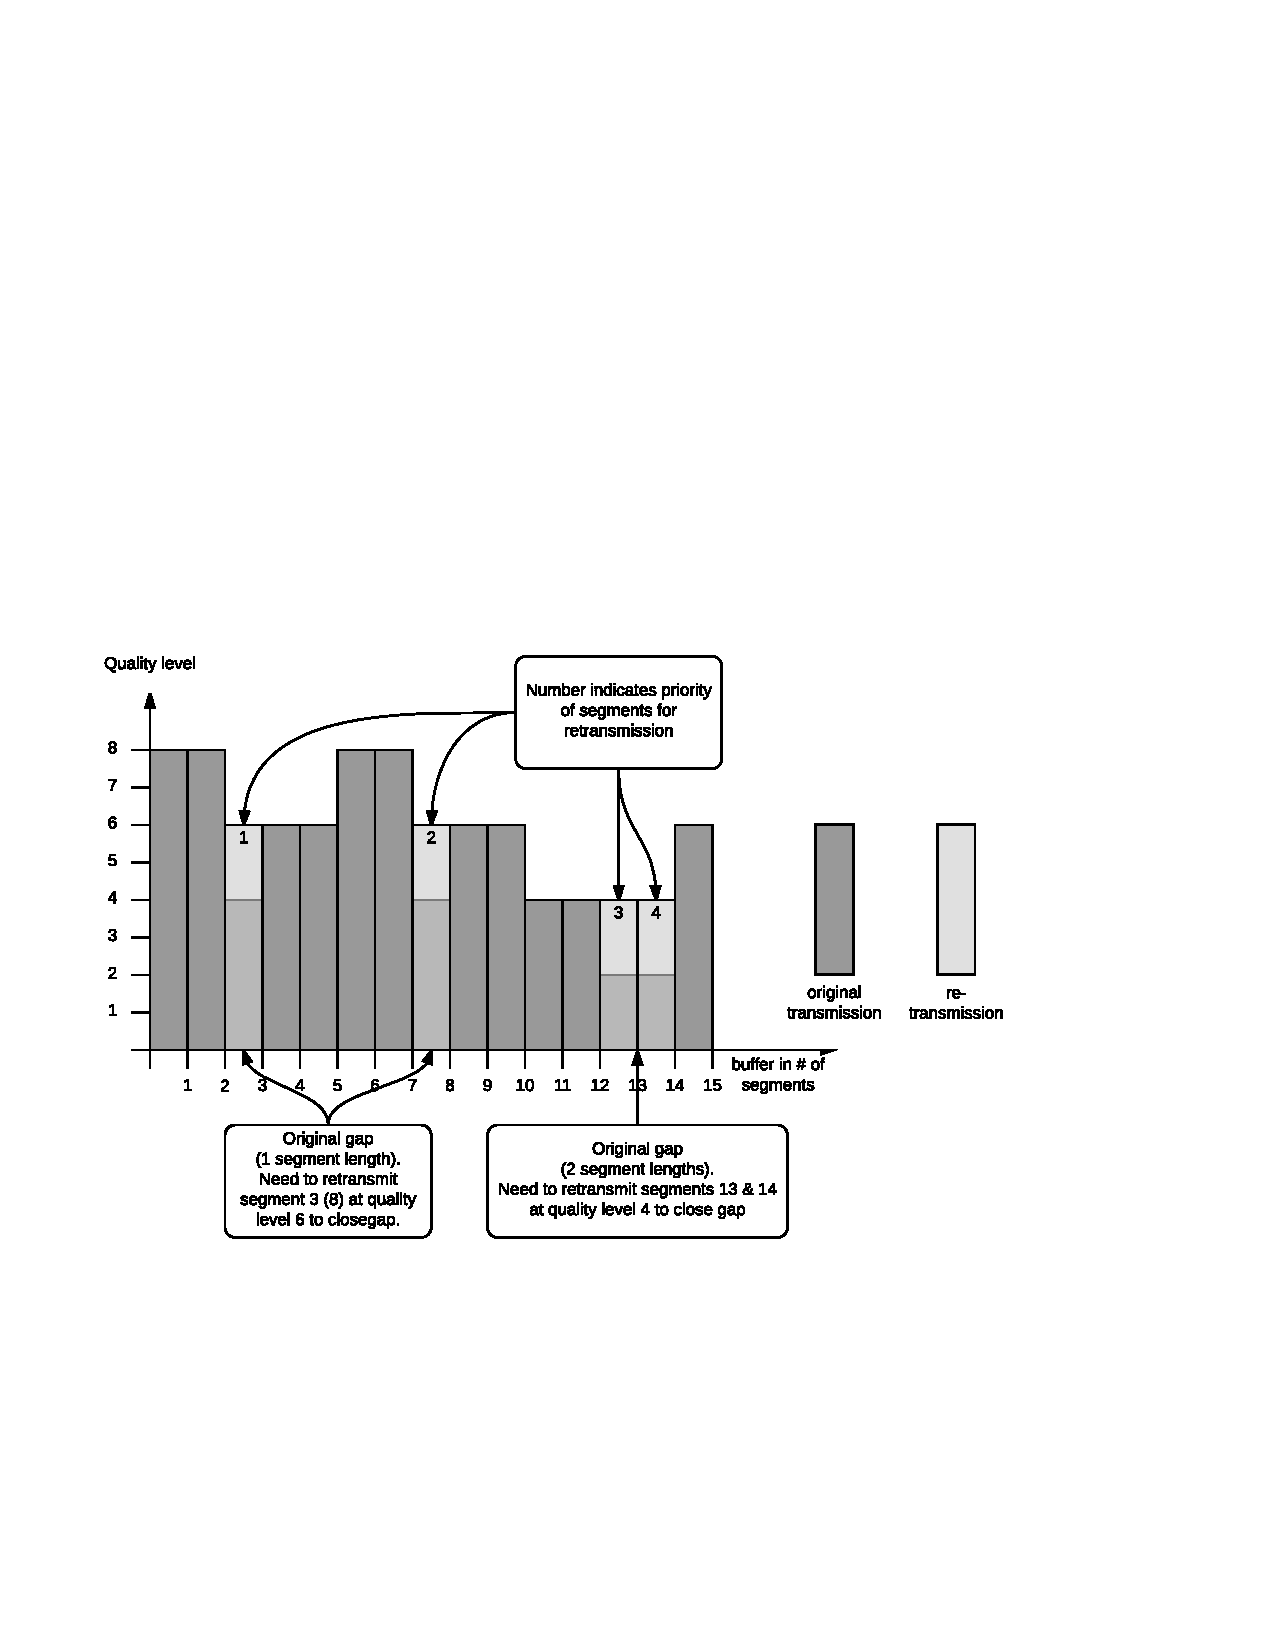
\includegraphics[scale=0.40, trim={0mm 100mm 0mm 90mm}] {figures/Retrans_example.pdf}
\caption{CDF for the number of sessions with one or more gaps for all sessions (orange) and mobile sessions (blue)}
\label{fig:gap_cdf}
\vspace{-12pt}
\end{figure}